\section{Einleitung}

	Vorverstädnis, Einleitung in die Arbeit

\section{Der Text: Mk 2,\ 1--12}

	\subsection{Übersetzung aus dem Urtext}

		\textit{Auf der Grundlage des Textes des \textsc{Novum Testamentum Graece}\footcite{NA28} wurde der Urtext übersetzt wie folgt:}

			\textsuperscript{Mk 2,\ 1} Und er kam nach einigen Tagen wieder nach Kapernaum und man hörte, dass er in einem Hause sei. \textsuperscript{2} Und es versammelten sich so viele, so daß kein Platz mehr war, auch nicht vor der Tür; und er sagte zu ihnen das Wort. \textsuperscript{3} Und sie kommen und bringen vor ihn einen Gelähmten, der von vieren getragen wurde. \textsuperscript{4} Und weil sie [ihn\footnote{Ergänzung durch d. Vf.}]  wegen der Volksmenge nicht zu ihm bringen können, deckten sie das Dach ab, wo er war, und nachdem sie es aufgegraben hatten, lassen sie das Bett hinunter, darin der Gelähmte lag. \textsuperscript{5a} Und weil Jesus ihren Glauben erkannte, sagt er zu dem Gelähmten:

			\textcolor{black}{\textsuperscript{5b} \textit{\frqq Kind, deine Sünden werden dir erlassen.\flqq} \textsuperscript{6} Es saßen dort aber auch einige der Schriftgelehrten und überlegten in ihren Herzen: \textsuperscript{7} \textit{\frqq Wer ist er, dass er dies sagt? Er lästert. Wer kann Sünden erlassen außer einem, der ist Gott?\flqq} \textsuperscript{8} Und weil Jesus sogleich in seinem Geist erkannte, was sie so bei sich überlegten, sagte er zu ihnen: \textit{\frqq Was überlegt ihr in euren Herzen?} \textsuperscript{9} \textit{Was ist leichter? Dem Gelähmten zu sagen: deine Sünden werden dir erlassen? Oder zu sagen: steh auf, nimm dein Bett und geh umher?} \textsuperscript{10} \textit{Damit ihr aber wisst, dass der Menschensohn Vollmacht hat, auf der Erde die Sünden zu erlassen --\flqq}}

			\textsuperscript{11} \textit{\frqq ich sage dir: steh auf, nimm dein Bett und geh in dein Haus.\flqq} \textsuperscript{12} Und er stand auf und, nachdem er sofort sein Bett genommen hatte, ging er vor allen hinaus, so daß alle staunten und den Gott verherrlichten indem sie sagten: \textit{\frqq etwas derartiges haben wir niemals gesehen.\flqq}

	\subsection{Textkritik}

		Der vorangehenden Übersetzung sowie der hier vorgelegten Exegese liegen die textkritischen Entscheidungen in Anhang 1 zugrunde.

\section{Literarkritik}

	\subsection{Einleitungsfragen}

		Das Markusevangelium entstand \glqq entweder \textit{kurz vor oder kurz nach 70 n. Chr.}\grqq, da sich Mk 13,\ 2.14 sowohl als Bezug auf die Zerstörung des jerusalemer Tempels durch die Römer als auch als entsprechende Prophezeiung verstehen lässt\footcite[269]{schnelle2013}.

		Sein Verfasser, der aufgrund der semitischen Färbung seiner Sprache vermutlich zweisprachig griechisch-aramäisch gewesen war\footcite[Cf.][275]{dschulnigg1986}, war wohl eher ein ansonsten unbekannter Christ mit dem Namen Markus\footcite[Cf.][267]{schnelle2013} als der Dolmetscher des Petrus, wie von Papias von Hierapolis berichtet\footcite[Cf.][266]{schnelle2013}. Die genaue Verfasserschaft bleibt aber letztlich unklar.

		Der Abfassungsort lässt sich aufgrund der vielen Latinismen\footcite[Cf.][268]{schnelle2013}\footcite[Cf.][277ff.]{dschulnigg1986} im Evangeliumstext auf Rom eingrenzen, wobei die Latinismen ebenfalls aufgrund der herrschenden römischen Weltmacht ihren Einzug in Mk gefunden haben könnten\footcite[Cf.][268]{schnelle2013}.

		Obschon der Abfassungsort Rom als gesichert gelten kann, ist gleichwohl der Adressat vermutlich nicht die römische Gemeinde gewesen. Der Adressat ...

	\subsection{Abgrenzung der Perikope}

		Nunmehr soll die Frage der Abgrenzung der Perikope im Markus-Evangelium behandelt werden.

		Nach hinten ist die Perikope abgegrenzt durch den erneuten Einsatz mit dem Bericht von Jesu Reise nach Kapernaum, es findet also ein Orts- und Zeitwechsel (\textit{\glqq nach einigen Tagen\grqq}) statt.

		Nach vorne ist die Perikope gleichfalls abgegrenzt durch ein Ortswechsel in V. 13: \textit{\glqq Und er ging wieder hinaus nahe des Sees...\grqq}.

	\subsection{Kontextanalyse}

		Gliederung Mk



		Verhältnis Perikope/Mk, Mk/Evangelien, Evangelien/NT, NT/Heilige Schrift

	\subsection{Gliederung der Perikope}

		Die Perikope wird in drei Abschnitte gegliedert:

		\paragraph{I.} Vv. 1--5a: Jesu Auftritt in Kapernaum, Predigt, Vorstellung des Gelähmten und Ansprache durch Jesus.

		\paragraph{II.} Vv. 5b--10: Sündenvergebung, Streitgespräch mit den Pharisäern.

		\paragraph{III.} Vv. 11--12: Erneute Ansprache Jesu, Aufstehen des Gelähmten, Staunen des Volkes.

	\subsection{Textpragmatik}

		Das Evangelium wurde geschrieben, als ...

		Der Verfasser wollte mit dem Evangelium wohl ... Dazu verwendetee er ..., um das Gefühl auszulösen ...

	\subsection{Grammatik und Syntax}

		Wortformen, Satzarten, Grammatik

	\subsection{Textsemantik}

		Wortschatz,

	\subsection{Quellenkritik, Synoptischer Vergleich}

		Alte Texte, wie vorliegend eines Evangeliums, müssen immer auch hinsichtlich ihrer Quellen befragt werden, was im Folgenden geschehen soll.

		In der Evangelienexegese ist ein Umstand besonders auffällig: Die Evangelien Matthäus, Markus und Lukas sind in hohem Maße literarisch von einander abhängig und stimmen in weiten Teilen inhaltlich und strukturell überein\footcite[Cf.][83]{niebuhr2011} -- daher man sie auch \textit{synoptische Evangelien} nennt --, wohingegen alle drei auch ihnen exklusiven Textbestand besitzen (sog. Sondergut) bzw. gegenüber den anderen Inhalte auslassen (sog. Lücken). Um das Verhältnis dieser drei synoptischen Evangelien untereinander besser beschreiben zu können, wurde die \textit{Zwei-Quellen-Theorie} entwickelt. Diese fußt zum einen wegen seines Alters auf der Priorität des Markus und zum anderen auch auf der so genannten Logienquelle.

		Bemerkenswert ist, dass \glqq die drei Evangelien sowohl im Wortbestand wie in der Anordnung einander am nächsten sind, wo sie mit dem [...] Markusevangelium parallel gehen\grqq\footcite[84]{niebuhr2011}; deshalb, und weil es als das älteste Evangelium angesehen wird\footcite[Cf.][210]{schnelle2013}, wird Mk als die \textit{erste} und wichtigste \textit{Quelle} der beiden betrachtet (\glqq Markuspriorität\grqq\footcite[84]{niebuhr2011}\footcite[ibid.]{schnelle2013}). Es wird angenommen, dass Mt und Lk wesentliche Inhalte von Mk übernommen und diesen womöglich verbessert haben\footcite[Cf.][213]{schnelle2013}.

		Bei dem verbleibenden Textbestand von Mt oder Lk, der also nicht Inhalt von Mk ist, gibt es eine zweite Schnittmenge, die sog. \textit{Logien-Quelle} (\textit{Q}), und welche die zweite Quelle darstellt. Es wird angenommen, dass es sich hierbei um wörtliche Aussprüche Jesu handelt.

		Es gibt ferner auch noch matthäisches bzw. lukanisches Sondergut, also Texte, die sich weder in Mk noch in Q finden\footcite[Cf.][216]{schnelle2013}, wobei man bei deren Einbeziehung dann eigentlich zu einer Vier-Quellen-Theorie gelänge.

		Die Zwei-Quellen-Theorie (eigentlich Vier-Quellen-Theorie) läßt sich also grafisch folgendermaßen darstellen\footcite[Grafik und Beschriftung entnommen aus][84]{niebuhr2011}:

		\begin{center}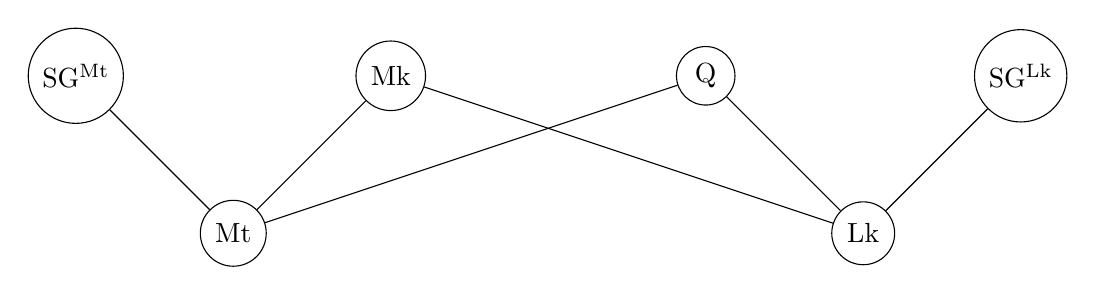
\begin{tikzpicture}[scale=2]
			% Knoten
			\node (Mk) at (3,1) [circle,draw] {Mk};
			\node (Q) at (5,1) [circle,draw] {Q};
			\node (Mt) at (2,0) [circle,draw] {Mt};
			\node (Lk) at (6,0) [circle,draw] {Lk};
			\node (SGLk) at (7,1) [circle,draw] {SG\textsuperscript{Lk}};
			\node (SGMt) at (1,1) [circle,draw] {SG\textsuperscript{Mt}};

			% Kanten
			\draw[-] (SGMt) to (Mt);
			\draw[-] (Mk) to (Mt);
			\draw[-] (Mk) to (Lk);
			\draw[-] (Q) to (Mt);
			\draw[-] (Q) to (Lk);
			\draw[-] (SGLk) to (Lk);
		\end{tikzpicture}\end{center}

		Ein Problem der Zwei-Quellen-Theorie ist aber, dass es durchaus auch markinisches Sondergut gibt. Dieses lässt sich nicht immer mit einer redaktionellen Tätigkeit von Mt oder Lk erklären. So lassen sich einige Auslassungen aus Gründen einer möglichen Anstößigkeit erklären, so etwa Mk 7 (Heilung eines Tauben) oder auch Mk 3 (Meinung der Verwandten, Jesus sei wahnsinnig). Das Fehlen des Gleichnisses von der selbstwachsenden Saat (Mk 4) bei Mt und Lk lässt sich so aber nicht begründen\footcite[Cf.][213]{schnelle2013}.

		Ein weiteres Problem der Zwei-Quellen-Theorie sind die sog. \textit{\glqq minor agreements\grqq} zwischen Mt und Lk gegen Mk, was auch ein Hauptgegenargument gegen die Zwei-Quellen-Theorie überhaupt ist\footcite[Cf.][84]{niebuhr2011}. Diese so genannten \textit{minor agreements} sind zum teil sprachliche

		Ein anderes Problem ist auch die so genannte \textit{lukanische Lücke}, also dass Lk den Stoff aus Mk 6,45--8,26 (der Seewandel bis zur Heilung des Blinden) vollständig ausgelassen hat. Hätte Lk das Markusevangelium in der heutigen Fassung vorgelegen, wäre dies kaum zu erklären\footcite[Cf.][213]{schnelle2013}.

		Ein letztes Problem wäre auch, dass Jesus wohl nicht griechisch sprach sondern wohl eher aramäisch. Eine griechische Logiensammlung mag es gegeben haben. Man müsste aber vor allem eine aramäische Logienquelle annehmen. Denkbar ist aber auch, dass die angenommene Logienquelle in sich nicht einheitlich ist\footcite[][]{schnelle2013}

		Es gab und gibt verschiedene Versuche, diese Probleme zu lösen, etwa durch Annahme, das heutige, kanonische Mk wurde hin zu einem eigeständigen oder als redaktionelle Version existierenden \glqq Deuteromarkus\grqq\ überarbeitet\footcite[Cf.][215f.]{schnelle2013} und um sein Sondergut gekürzt, wobei DtoMk wiederum die Grundlage für Mt und Lk gewesen sein könnte.

		Zusammenfassend läßt sich sagen, dass die Zwei-Quellen-Theorie aufgrund der Vielzahl ihrer Probleme und der dadurch erzwungenen Annahmen nicht stärker oder überzeugender wird. Dennoch ist sie der aktuelle Quasi-Standard in der exegetischen Wissenschaft. Wenn sie schon nicht alle Fragen beantwortet und aufgrund der vielfältigen Annahmen eben nicht besonders belastbar ist, so ist sie doch hilfreich, die Beziehungen der Synoptiker untereinander wenigstens ansatzweise zu verstehen.

		Dennoch wollen wir die vorliegende Perikope mit ihren Parallelstellen bei den beiden anderen Synoptikern vergleichen und wenden hierfür die Zwei-Quellen-Theorie an. Wo möglich wird auch direkt die (vermutete) Quelle notiert.

		\begin{table}[h]
		\begin{tabular}{|l|l|l|l|l|}
		\hline \textbf{Abschnitt} & \textbf{Mt 9, 9--13} & \textbf{Mk 2, 1--12} & \textbf{Lk 5, 27--32} & \textbf{Quelle} \\\hline\hline
		          &    &    &    &    \\\hline
		          &    &    &    &    \\\hline
		          &    &    &    &    \\\hline
		          &    &    &    &    \\\hline
		          &    &    &    &    \\\hline
		          &    &    &    &    \\\hline
		          &    &    &    &    \\\hline
		          &    &    &    &    \\\hline
		          &    &    &    &    \\\hline
		          &    &    &    &    \\\hline
		          &    &    &    &    \\\hline
		          &    &    &    &    \\
							\hline
		\end{tabular}
		\end{table}

	\subsection{Einheitlichkeit}

		Schriftgelehrte!? Einfügung eines Streitgesprächs? Einfügung der Vv. 6--10 \footcite[Cf.][29f.]{schweizer1998}

		Auffällig ist, dass die Schriftgelehrten plötzlich und unvermittelt in der Geschichte auftauchen. So ist in den Vv. 1--5a überhaupt nicht von ihnen die Rede. Erst mit V. 6 werden sie erwähnt. Auch in Mk 1 gibt es noch kein solches Streitgespräch.

		Ebenso auffällig ist der doppelte Anhub Jesu zur Anrede des Gelähmten: erstens mit \glqq Kind\grqq, V. 5b, und später erneut mit \glqq Ich sage dir...\grqq, V. 11.

		Die vorliegende Perikope ist mithin nicht einheitlich

	\subsection{Narrative Analyse}

		Der Handlungsablauf in der Perikope stellt sich dar wie folgt:

		\begin{enumerate}
			\item (V. 1) Jesus kommt nach Kapernaum.
			\item (V. 2) Es versammelten sich viele, Jesus predigt ihnen.
			\item (Vv. 3f.) Sie bringen ihm den Gelähmten und decken dafür das Dach ab.
			\item (V. 5a) Jesus spricht den Gelähmten an.
			\item (V. 5b) Jesus vergibt dem Gelähmten seine Sünden.
			\item (Vv. 6ff.) Die Schriftgelehrten beschuldigen Jesus, Jesus antwortet im Stil eines Streitgespräches.
			\item (Vv. 11, 12a.) Jesus fordert den Gelähmten zum Aufstehen und Gehen auf; er steht auf und geht.
			\item (V. 12b) Das Volk staunt.
		\end{enumerate}

\section{Formgeschichte}

	\subsection{Traditionsgeschichte}

	\subsection{Redaktionsgeschichte}

	 Die Perikope besteht, wie bereits oben in der Übersetzung und auch bei der Gliederung der Perikope angedeutet, zumindest aus zwei Schichten: Die erste und ursprünglichere Schicht erstreckt sich also über die Vv. 1--5(a).11--12 und umfasst das Heilungswunder. Die zweite und jüngere Schicht erstreckt sich entsprechend über die Vv. 5(b)--10 und umfasst das, wie noch zu zeigen ist, nachträglich eingefühte Streitgespräch zwischen Jesus und den Schritgelehrten.

	\subsection{Gattungsbestimmung}

		Wundergeschichte

		eingebettet: Apophthegma

		Chrie? "Wer, was, warum, gegen, ähnlich, Beispiele, Zeugen?"

\section{Begriffs- und Motivgeschichte, Historischer Zusammenhang}

	\subsection{Religionsgeschichtlicher Vergleich}

	\subsection{Historischer Zusammenhang}

		70 n Christus

		Jüdischer Krieg

		Belagerung Jerusalems

		Zerstörung des jerusalemer Tempels

		Eroberung Jerusalems

	\subsection{Begriffs- und Motivgeschichte}

		Dächer in der Antike

		Lähmung als Krankheit

		{\ibygr{lalein ton logon}} = er redet das Wort, also höchstens das Evangelium, nicht den Logos \footcite[Cf.][16, 33]{wellhausen1903Mk}

		Streitgespräch

		Wundererzählung / Heilungswunder

	\subsection{Rückfrage nach Jesus}

		Logienquelle?

\section{Interpretation}

	\subsection{Auslegung}

	\subsection{Christologie bei Markus}

	\subsection{Ausblick}

		Wert für die Verkündigung
